\documentclass[a4paper, titlepage,12pt]{article}

\usepackage[margin=3.7cm]{geometry}
\usepackage[utf8]{inputenc}
\usepackage[T1]{fontenc}
\usepackage[swedish,english]{babel}
\usepackage{csquotes}
\usepackage[hyphens]{url}
\usepackage{amsmath,amssymb,amsthm, amsfonts}
\usepackage[backend=biber,citestyle=ieee]{biblatex}
\usepackage[yyyymmdd]{datetime}
\usepackage{titlesec} 
\usepackage{graphicx}
\usepackage{listings}

\usepackage{xcolor}
\definecolor{codegreen}{rgb}{0,0.6,0}
\definecolor{codepurple}{rgb}{0.5,0,0.5}
\definecolor{backcolor}{rgb}{0.97,0.97,0.97}

\usepackage[backend=biber,citestyle=ieee]{biblatex}
\addbibresource{./literature.bib}

\lstdefinestyle{mystyle}{
	commentstyle=\color{codegreen},
	keywordstyle=\color{magenta},
	numberstyle=\color{gray}\ttfamily\footnotesize,
	backgroundcolor=\color{backcolor},
	basicstyle=\ttfamily\footnotesize,
	stringstyle=\color{codepurple},
	numbers=left,
	tabsize=4
}

\lstset{style=mystyle}


\iffalse
\titleformat{\subsection}[runin]
  {\normalfont\large\bfseries}{\thesubsection}{1em}{}
\titleformat{\subsubsection}[runin]
  {\normalfont\normalsize\bfseries}{\thesubsubsection}{1em}{}
\fi

\title{Performance Analysis and Simulation of Communication Systems: Project A}

\author{Adam Temmel (adte1700) \& Fredrik Sellgren (frse1700)}

\begin{document}
	\maketitle
	\section{PRNG and Random Variables}
		\subsection{Create a function that implements a linear congruential generator (LCG), accepting as input the parameters: seed, m, a,and c.}
		We implemented our LCG as a class in order to keep it somewhat similiar to the STL generators. The code used is as follows:

		\begin{figure}[h!]
			\begin{lstlisting}[language=c++]
class Lcg {
public:
	using seed_t = uint32_t;

	Lcg(seed_t seed, seed_t m = 100, seed_t a = 13, 
		seed_t c = 1) 
		: seed(seed), m(m), a(a), c(c) {}

	seed_t operator()() {
		seed = ((a * seed) + c) % m;
		return seed;
	}

	// These are kept public to make it easier to change 
	// them later in the lab, a more authentic generator
	// would probably keep them private.
	seed_t seed, m, a, c;
};
			\end{lstlisting}
			\caption{LCG Class}
			\label{fig:lcgimpl}
		\end{figure}



		\subsection{Generate 1000 values uniformly distributed in the range [0,1] using your PRNG. For this case use m=100, a=13 c=1and seed =1;}

		The code used to generate 100 uniformly distributed values is presented in \textit{\ref{fig:uniformcode}}.

		\begin{figure}[h!]
			\begin{lstlisting}[language=c++]
template<typename T>
double normalize(T x, T min, T max) {
	return static_cast<double>(x - min) 
		/ static_cast<double>(max - min);
}

void testPrng() {
	Lcg lcg(1);

	auto urv = CreateObject<UniformRandomVariable> ();
	constexpr size_t n = 1000;

	std::vector<double> ourResults(n);

	std::generate(ourResults.begin(), ourResults.end(), 
			[&]() {
		return normalize(lcg(), 0u, lcg.m);
	});

	std::vector<double> theirResults(n);

	std::generate(theirResults.begin(), theirResults.end(), 
			[&]() {
		return urv->GetValue(0., 1.);
	});

	{
		std::ofstream ourFile("our_results.txt");
		for(auto f : ourResults) {
			ourFile << f << ' ';
		}
	}

	{
		std::ofstream theirFile("their_results.txt");
		for(auto f : theirResults) {
			theirFile << f << ' ';
		}
	}
}
			\end{lstlisting}
			\caption{Code used to write 1000 uniformly generated values from each generator to disk}
			\label{fig:uniformcode}
		\end{figure}
		\pagebreak

		\subsection{Compare the distribution of your values with the distribution of values generated using the \\
		\lstinline{UniformRandomVariable()} of ns-3.}
		Two histograms comparing our generator to the Ns3 generator are visualized in \textit{figure \ref{uniform_plots}}.
		\begin{figure}[h!]
			\begin{center}
				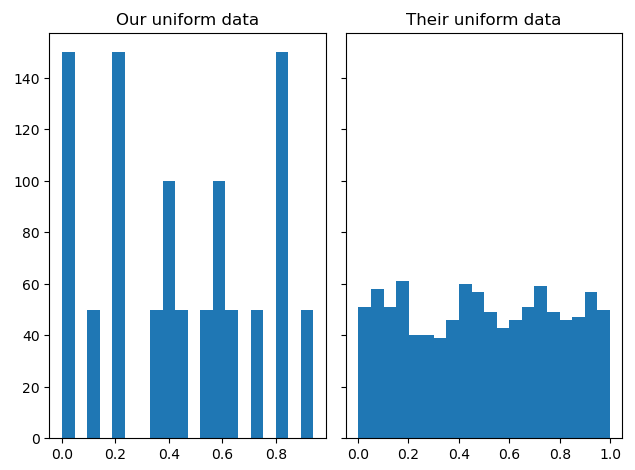
\includegraphics[scale=0.8]{./uniform_histogram_plot.png}
				\caption{The corresponding plots gathered from the data above}
				\label{uniform_plots}
			\end{center}
		\end{figure}
		\subsection{Comment on the difference in the results and propose values of m, a, and c which gives you better results.}
		The main issue we found with the parameters given comes from the divisor used when performing the modulus operation, $m$. As $m$ was initially set to $100$, we are guaranteed to only generate numbers in $[0, 99]$. It then follows that our generator can only generate $100$ different values. This might be enough for some cases, but seeing as we wish to normalize it into a continuous value between $[0, 1]$, the lack of representable numbers provided by the generator will have a negative impact on the final result. As such, it is in our interest to increase the divisor. One suggested method of improving the generator is to use a divisor that is a power of $2$, such as $2^{32}$ or $2^{64}$ combined with keeping $c$ at $0$\cite{artofprogramming}. Another possible competitor for good divisors are the \emph{Mersenne Primes}, such as $2^{32}-1$ or $2^{64}-1$\cite{mersenne}, which also happens to be exactly the fix we implemented. This improvement proved to make a noticeable difference, which is illustrated in \textit{figure~\ref{improved_uniform_plots}}.
		\begin{figure}[h!]
			\begin{center}
				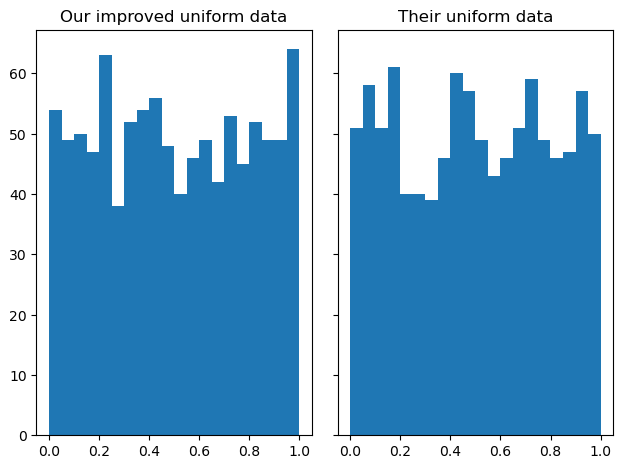
\includegraphics[scale=0.8]{./improved_uniform_histogram_plot.png}
				\caption{Our improved generator compared to the Ns3 generator}
				\label{improved_uniform_plots}
			\end{center}
		\end{figure}
		\subsection{What PRNG does ns-3 use?  What method does ns-3 use to generate a normal random variable?}
		The PRNG that is used in Ns3 is the MRG32k3a generator\cite{ns3-random}. The underlying implementation comes from Pierre L'Ecuyer's (among others) random number generator package\cite{random-pierre}.
		MRG32k3a implements a way to generate random numbers capable of being separated into disjoint substreams that are independent from one another. Ns3 states that the total period of the generator is $3.1 \cdot 10^{57}$\cite{ns3-random}.
		\subsection{Using the \lstinline{time} system command of Linux compare the execution time for the generation of the uniform distribution using your function and ns-3 function}

		\begin{figure}[h!]
			\begin{center}
			\begin{lstlisting}
# our class: 
time ./waf --run scratch/project  2.54s user 0.20s 
system 107% cpu 2.547 total
# their class: 
time ./waf --run scratch/project  2.59s user 0.17s 
system 107% cpu 2.556 total
			\end{lstlisting}
			\caption{The results from timing a program that generated 1000 random numbers using \lstinline{time}}
			\end{center}
		\end{figure}
		\pagebreak
			As we can see, our implementation is slightly faster (around $0.01$ seconds) than the Ns3 implementation.
		\subsection{Write a second function that generates an exponential distribution with mean $\beta>0$ from a uniform distribution generated using the LCG; Choose one of the methods for generating RV covered in the course and motivate your choice with respect to the specific task.}
		The course brought up the concept of \emph{The Inverse Transform Algorithm}. It operates as follows:
		\begin{enumerate}
			\item Generate $u \in U(0, 1)$.
			\item Define a function $F(X)$, which represents the distribution of the random data you wish to generate. In our case, this was an exponential distribution, so something akin to $F(X) = 1 - e^x$.
			\item Solve the equation $F(X) = U$ for $X$, finding the inverse $X = F^{-1}(U)$. In our case, $F^{-1}(U) = -ln(1-U)$.
			\item By inserting $u$ into $F^{-1}$, we can now convert a uniform $[0, 1]$ variable into the desired distribution.
		\end{enumerate}
		We argued that the Inverse Transform Algorithm was the most appropriate method for the task, as we have a specific target function we wish to reach, which rules out a few of the alternative methods. Furthermore, all the steps involved in this algorithm are arguably less complex compared to, say, The Rejection Method.
		\begin{figure}[h!]
			\begin{lstlisting}[language=c++]
double expDist(double value, double lambda) {
	return -log(1 - value) / lambda;
}
			\end{lstlisting}
			\caption{Resulting code after implementing the Inverse Function Transform}
			\label{fig:invfunctrans}
		\end{figure}
			
		\subsection{Compare your exponential distribution with ns-3 \lstinline{ExponentialRandomVariable()} and the theoretical expression of the probability density function.}
		\begin{figure}[h!]
			\begin{center}
				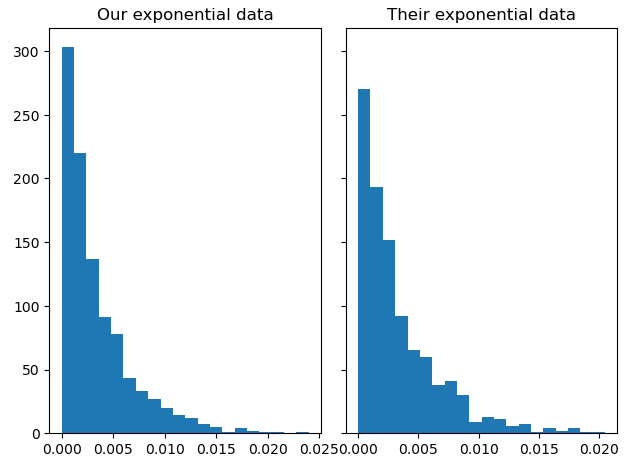
\includegraphics[scale=0.8]{./exponential_histogram_plot.png}
				\caption{Our exponentially distributed generator compared to the Ns3 counterpart}
				\label{exp_plots}
			\end{center}
		\end{figure}
		As is illustrated in \textit{figure~\ref{exp_plots}}, the two generators ended up performing on a somewhat equal level.

		\section*{Citations}
			\printbibliography
\end{document}
